\chapter{計量、膨張、そして最初の宇宙論}

前回の講義の終わりに、われわれはローレンツ不変な波動方程式に到達し、マクスウェル方程式を時空の形で書く準備をしていた。ここで聴衆からの質問が、重力へ移る前に有用な警告を与えてくれる。すなわち、対称性だけによって物理理論のどこまでが決定されるのか、という問いである。答えは断固としている。多くを決定するが、すべてではない。ローレンツ不変性は可能な法則に対する強力なフィルターである。しかしそれは、残りの物理的仮定や実験の代わりにはならない。

\section{対称性が決定しないもの}

\begin{classroomqa}
\audiencequestion{電場と磁場がローレンツ変換の下でともに変換することが分かったなら、マクスウェル方程式は相対性理論だけから導かれるのか。}
\lecturerresponse{否である。相対性理論は方程式の形を制約するが、その構成には方程式の線形性、その導関数の低い次数、場の変換の仕方、そして実験的情報も用いられる。それらの追加の要素がなければ、多くのローレンツ共変な場の方程式が依然として可能であろう。}
\end{classroomqa}

冒頭の議論にとって、それらの追加の仮定のうち最も重要なものは線形性である。\(A(x,t)\) が線形な場の方程式の解ならば、任意の定数 \(\lambda\) に対して \(\lambda A(x,t)\) もまた解である。\(A\) と \(B\) が解ならば、
\begin{equation}
  C(x,t)=A(x,t)+B(x,t).
  \label{eq:superposition}
\end{equation}
もまた解である。これが重ね合わせの原理である。2つの源のない電磁波は互いに交差しても変化せずに出てくる。それらは物質的な物体のように直接衝突するのではない。それらは荷電物質を通じて間接的に相互作用しうる。なぜなら各々の波は電荷を動かし、動く電荷は放射するからであるが、真空の場の方程式そのものは線形である。

\begin{figure}[H]
\centering
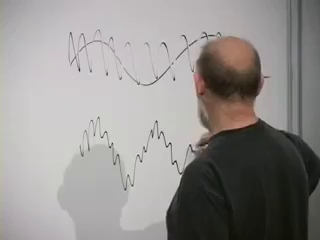
\includegraphics[width=0.64\textwidth]{lecture_08_figure_01.png}
\caption{重ね合わせの議論の際に黒板に示された2つの波のプロファイル。それらの和もまた許される源のない波である。}
\lectureframe{00:05:30}
\end{figure}

調和振動子はこの代数を透明にする。次を仮定する。
\begin{equation}
  m\ddot x=-kx.
  \label{eq:linear-oscillator}
\end{equation}
\(x_1\) と \(x_2\) が \eqref{eq:linear-oscillator} を解くならば、
\begin{equation}
  m(\ddot x_1+\ddot x_2)
  =-k(x_1+x_2),
\end{equation}
であるから、\(x_1+x_2\) は解である。しかし非線形項を加えると、
\begin{equation}
  m\ddot x=-kx+p x^2,
  \label{eq:nonlinear-oscillator}
\end{equation}
和はもはや成り立たない。
\begin{equation}
  (x_1+x_2)^2=x_1^2+x_2^2+2x_1x_2.
\end{equation}
交差項 \(2x_1x_2\) は2つの別々の方程式には対応するものがない。2つの運動は今や互いに影響を及ぼし合う。

\begin{figure}[H]
\centering
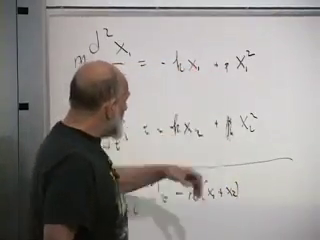
\includegraphics[width=0.73\textwidth]{lecture_08_figure_02.png}
\caption{分離した振動子の方程式を、それらの和の方程式と比較する。二次の項によって、重ね合わせを破る余分な交差項が現れる。}
\lectureframe{00:10:10}
\end{figure}

この例は、宇宙論の議論を通じて有効であり続ける方法論上の要点を確定する。対称性は、どの量が組み合わされうるか、どの方程式が許されるかを教える。力学と観測が、許された方程式のうち自然がどれを用いるかを教える。

\section{幾何学としての間隔}

ここで電磁気学を離れ、一般相対性理論と宇宙論への短い道筋に入る。出発点となる対象は、隣り合う事象の間の間隔である。ある事象を4つの座標\(x^\mu\)でラベルし、近くの事象を\(x^\mu+dx^\mu\)でラベルする。慣性系のデカルト座標において、\(c=1\)および\((+,-,-,-)\)の規約を用いると、
\begin{equation}
  d\tau^2
  =dt^2-dx^2-dy^2-dz^2
  =dx^\mu dx_\mu
  =\eta_{\mu\nu}\,dx^\mu dx^\nu.
  \label{eq:minkowski-interval}
\end{equation}
不変なのは量\(d\tau^2\)であり、座標差のどれか一つではない。ローレンツ変換は\(dt,dx,dy,dz\)を変化させるが、この二次の組み合わせは保つ。したがって特殊相対性理論は、ミンコフスキー時空の幾何学として読むことができる。

\begin{figure}[H]
\centering
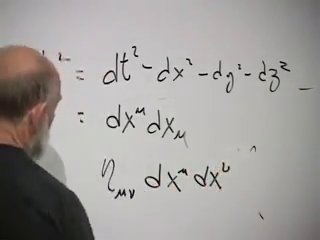
\includegraphics[width=0.72\textwidth]{lecture_08_figure_03.png}
\caption{ミンコフスキー間隔を、成分表示、縮約された添字表示、計量テンソル表示で順に書いたもの。}
\lectureframe{00:14:50}
\end{figure}

\eqref{eq:minkowski-interval} の単純さは座標に依存する。平らな平面でさえ、賢明でないラベルの付け方をすれば見慣れない係数を得る。\(x\) をセンチメートルで測り、\(y\) をメートルで測るとする。物理的な変位に対して、
\begin{equation}
  ds^2=dx^2+\left(\frac{dy}{100}\right)^2
      =dx^2+10^{-4}dy^2.
  \label{eq:mixed-units}
\end{equation}
因子 \(10^{-4}\) は曲率について何も語らない。それは単に単位間の換算を行うだけである。

\begin{figure}[H]
\centering
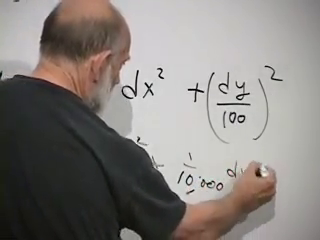
\includegraphics[width=0.59\textwidth]{lecture_08_figure_04.png}
\caption{一方の軸をセンチメートル、他方をメートルで記述した平らな平面。等しくない計量係数は曲率ではなく単位を表している。}
\lectureframe{00:20:10}
\end{figure}

斜交座標では混合項が加わる。2次元では、最も一般的な局所二次形式は
\begin{align}
  ds^2
  &=a_{11}\,dx^2+a_{12}\,dx\,dy\notag\\
  &\quad+a_{21}\,dy\,dx+a_{22}\,dy^2,
  \qquad a_{12}=a_{21}.
  \label{eq:quadratic-form}
\end{align}
と書ける。通常の微分は可換であるから、\(dx\,dy=dy\,dx\)であり、係数配列の対称部分のみが寄与する。係数をまとめて行列
\begin{equation}
  g=
  \begin{pmatrix}
    a_{11} & a_{12}\\
    a_{21} & a_{22}
  \end{pmatrix}.
  \label{eq:metric-matrix}
\end{equation}
を得る。この行列が\emph{計量}である。これは座標差を物理的な間隔へ変換する局所的な規則である。

\begin{figure}[H]
\centering
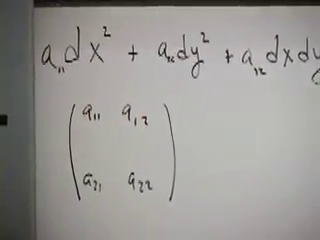
\includegraphics[width=0.71\textwidth]{lecture_08_figure_05.png}
\caption{二次微分形式と、その対称な\(2\times2\)係数行列。この行列が計量として同定される時点でのものである。}
\lectureframe{00:24:07}
\end{figure}

一様な矩形格子または斜交格子では、係数は一定になる。座標線が曲がったり、互いに密集したり、離れていったりすると、下にある面が平坦なままであっても、それらの係数は位置の関数になる。一般の時空の表記は
\begin{equation}
  ds^2=g_{\mu\nu}(x)\,dx^\mu dx^\nu.
  \label{eq:general-metric}
\end{equation}

\begin{figure}[H]
\centering
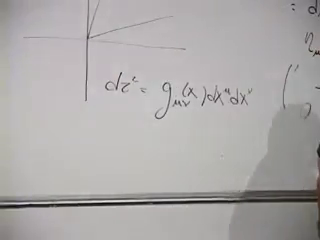
\includegraphics[width=0.66\textwidth]{lecture_08_figure_06.png}
\caption{座標格子が点ごとに変化することを許した後の、一般の位置依存計量。}
\lectureframe{00:28:10}
\end{figure}

指定された座標系で\(g_{\mu\nu}\)がわかれば、局所的な距離、時間、角度が決まり、それによって幾何が決まる。逆は一意ではない。一つの幾何には無限に多くの座標記述があり、したがって座標変換で互いに関係づけられる無限に多くの係数関数の配列がある。

\section{座標の複雑さと内在的曲率}

ここで、複雑な計量と曲がった空間を区別しなければならない。紙を引き伸ばさずに円筒に丸める。部屋の中での見え方は変わるが、紙の内部で測られるすべての距離は同じままである。紙に閉じ込められた生き物は、いかなる内在的測定によっても、その曲げを検出できない。それは外在的な曲げであり、ここで意味している曲率ではない。

半球は異なる。引き伸ばしたり、破いたり、圧縮したりせずに平らに押しつぶすことはできない。地球の平らな地図は、距離、面積、角度、またはそれらの何らかの組み合わせを歪めざるを得ない。この障害は内在的であり、周囲の次元を覗き込むことなく検出できる。

極座標は不可欠な平坦な反例を与える。平面上では、無限小の動径方向の変位の長さは\(dr\)であり、半径\(r\)における角度変位\(d\theta\)の長さは\(r\,d\theta\)である。したがって
\begin{equation}
  ds^2=dr^2+r^2d\theta^2,
  \qquad
  g_{\text{polar}}=
  \begin{pmatrix}
    1&0\\
    0&r^2
  \end{pmatrix}.
  \label{eq:polar-metric}
\end{equation}
係数\(r^2\)は平面全体で変化するが、平面は平坦である。変数変換
\begin{equation}
  x=r\cos\theta,\qquad y=r\sin\theta
\end{equation}
は一定の計量\(ds^2=dx^2+dy^2\)を返す。

\begin{figure}[H]
\centering
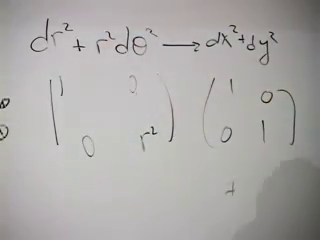
\includegraphics[width=0.70\textwidth]{lecture_08_figure_07.png}
\caption{極座標計量とそのデカルト計量への回帰。左側の位置依存行列は依然として平坦な平面を記述している。}
\lectureframe{00:39:20}
\end{figure}

\begin{classroomqa}
\audiencequestion{極座標における角度距離にはサインが含まれるべきか。}
\lecturerresponse{平面上では含まれない。そこでは弧の長さは
\(r\,d\theta\)である。サインは球面上に現れ、そこでは緯度円の半径は\(R\sin\theta\)である。}
\end{classroomqa}

半径\(R\)の球を考える。\(\theta\)を北極から測った極角、\(\phi\)を方位角とする。子午線方向の歩みの長さは\(R\,d\theta\)である。極角\(\theta\)において、緯度円の半径は\(R\sin\theta\)であるから、方位角方向の歩みの長さは
\(R\sin\theta\,d\phi\)である。局所的なピタゴラスの定理により
\begin{align}
  ds^2
  &=R^2\left(d\theta^2+\sin^2\theta\,d\phi^2\right),
  \label{eq:sphere-metric}\\
  g_{\text{sphere}}=
  &\begin{pmatrix}
    R^2&0\\
    0&R^2\sin^2\theta
  \end{pmatrix}.
\end{align}

\begin{figure}[H]
\centering
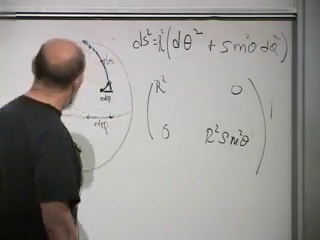
\includegraphics[width=0.72\textwidth]{lecture_08_figure_08.png}
\caption{球、その角度線素、および対応する計量行列。\(\sin^2\theta\)因子は緯度円が縮むことを記録している。}
\lectureframe{00:45:15}
\end{figure}

\begin{figure}[H]
\centering
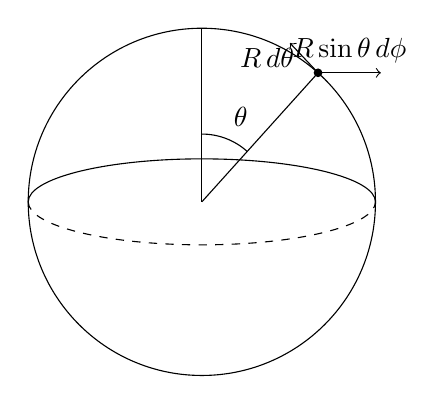
\begin{tikzpicture}[scale=1.05]
  \draw (0,0) circle (2.1);
  \draw[dashed] (-2.1,0) arc (180:360:2.1 and 0.52);
  \draw (2.1,0) arc (0:180:2.1 and 0.52);
  \coordinate (P) at (48:2.1);
  \fill (P) circle (1.5pt);
  \draw (0,0) -- (0,2.1);
  \draw (0,0) -- (P);
  \draw (0,0.82) arc (90:48:0.82);
  \node at (0.47,1.03) {\(\theta\)};
  \draw[->] (P) -- ++(-0.34,0.36)
    node[midway,left] {\(R\,d\theta\)};
  \draw[->] (P) -- ++(0.76,0)
    node[midway,above] {\(R\sin\theta\,d\phi\)};
\end{tikzpicture}
\caption{\eqref{eq:sphere-metric}を得るために用いた局所的な微分の脚の明快な再構成。}
\end{figure}

\eqref{eq:sphere-metric}を一定のユークリッド行列に変える大域的な座標変換は存在しない。二次元の観測者はこれを内在的に発見できる。測地線から作られた十分に大きな三角形の角の和は\(180^\circ\)より大きい。したがって、有用な判定基準に到達した。係数が変化することは、それ自体では曲率を意味しない。曲率とは、考察対象の領域全体で計量を一定にする座標を見つけることへの障害である。

\section{曲がった時空から宇宙論へ}

一般相対性理論は、時空自体がこの内在的曲率を持つことを許す。位置依存の\(g_{\mu\nu}\)は、極座標の場合のように、依然として座標の産物でありうるが、真に曲がった時空では、いかなる座標変換もその変化を大域的に取り除かない。

\begin{figure}[H]
\centering
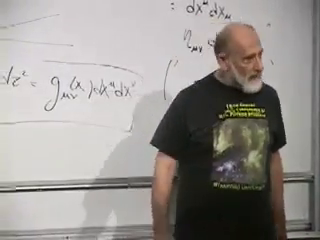
\includegraphics[width=0.70\textwidth]{lecture_08_figure_09.png}
\caption{特殊な座標の例から一般の時空線素\(ds^2=g_{\mu\nu}(x)dx^\mu dx^\nu\)への移行。}
\lectureframe{00:48:40}
\end{figure}

アインシュタイン方程式の完全な機構を試みることはしない。代わりに、宇宙論に適した幾何に注意を限定する。空間は十分に大きなスケールで一様であるとされ、一方で幾何は時間とともに変化しうる。一様とは、ある場所が別の場所から区別されないことを意味する。平坦であることを意味しない。球面上のすべての点は等価であるが、球面は曲がっている。また、あらゆるスケールで特徴がないことを意味するのでもない。

\begin{classroomqa}
\audiencequestion{銀河が集団、板、フィラメントを形成しているのに、なぜ宇宙は一様でありうるのか。}
\lecturerresponse{この主張は粗視化されたスケールに関するものである。恒星、銀河、銀河団は強く非一様である。数億光年にわたる領域を比較すると、それらの構造は一様な分布へと平均化される。宇宙原理は経験的な作業仮説であり、論理的必然ではない。宇宙背景における方向依存の差を含む、十分に大きな系統的差異があれば、それを反証しうる。}
\end{classroomqa}

この講義における第二の大規模な仮定は、空間的な平坦性である。固定された宇宙時刻において、十分に大きな三角形はユークリッド的に見える。すなわち、その角度の和は\(180^\circ\)となる。これは三次元空間の幾何学についての主張であり、まだ四次元時空の曲率についてのものではない。

\begin{classroomqa}
\audiencequestion{宇宙論的距離だけ離れた点にとって、それらの光が異なる時刻に我々に届くのだから、同時性とは何を意味するのか。}
\lecturerresponse{遠方の銀河の間に棒を置くことも、それらを瞬時に調べることもできない。我々は信号を後になって受け取り、時空模型の内部で放出事象の幾何学を再構成する。この手続きは間接的であるが、天文学における多くの幾何学的測定も同様である。平坦性とは、再構成された大きな三角形が、調査されたスケールにおいて検出可能な角度の過剰も不足も示さないことを意味する。}
\end{classroomqa}

\section{共動座標とスケール因子}

銀河の大規模な流れの上に描かれたデカルト格子を想像せよ。格子が膨張するにつれて、各銀河はその座標ラベルを保つ。そのラベルはメートル単位の距離ではなく、住所である。時間に依存する変換因子が、座標の隔たりを物理的な隔たりに変える。

\begin{figure}[H]
\centering
\begin{tikzpicture}[>=Latex,scale=0.86]
  \foreach \x in {0,0.65,1.3,1.95,2.6} {
    \draw[gray!65] (\x,0) -- (\x,2.2);
  }
  \foreach \y in {0,0.55,1.1,1.65,2.2} {
    \draw[gray!65] (0,\y) -- (2.6,\y);
  }
  \fill[blue!65!black] (0.65,0.55) circle (2pt);
  \fill[red!70!black] (1.95,1.65) circle (2pt);
  \node[below] at (1.3,-0.2) {comoving labels at \(t_1\)};
  \draw[->,very thick] (3.0,1.1) -- (4.0,1.1)
    node[midway,above] {\(a(t)\) grows};
  \foreach \x in {4.4,5.5,6.6,7.7,8.8} {
    \draw[gray!65] (\x,0) -- (\x,2.2);
  }
  \foreach \y in {0,0.55,1.1,1.65,2.2} {
    \draw[gray!65] (4.4,\y) -- (8.8,\y);
  }
  \fill[blue!65!black] (5.5,0.55) circle (2pt);
  \fill[red!70!black] (7.7,1.65) circle (2pt);
  \node[below] at (6.6,-0.2) {same labels at \(t_2\)};
\end{tikzpicture}
\caption{共動的な住所は固定されたままであり、一方で座標格子の物理的な間隔は増大する。}
\end{figure}

空間的な一様性は、与えられた時刻においてどこでも同じ変換因子を要求する。空間的な平坦性は、計量の空間部分がデカルト的であることを許す。結果として得られる線素は
\begin{equation}
  d\tau^2
  =dt^2-a^2(t)\left(dx^2+dy^2+dz^2\right).
  \label{eq:flrw-flat}
\end{equation}
である。これは共動座標における空間的に平坦で一様な宇宙論的計量である。\(x,y,z\)を無次元に選び、\(a(t)\)に長さの単位を与えてもよい。別の規約では、次元を座標に押し込み、\(a\)を無次元にすることもできる。重要なのは積だけである。

\begin{figure}[H]
\centering
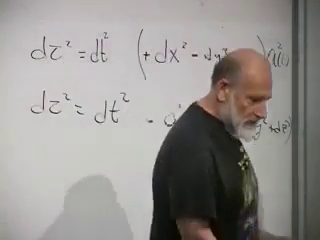
\includegraphics[width=0.76\textwidth]{lecture_08_figure_10.png}
\caption{黒板で完成された、空間的に平坦な宇宙論的計量。共通因子\(a^2(t)\)が三つの空間方向すべてに掛かっている。}
\lectureframe{01:03:15}
\end{figure}

もし\(a\)が定数であれば、\(x,y,z\)を再スケールすることによってそれを吸収でき、\eqref{eq:flrw-flat}は異なる単位での通常のミンコフスキー時空となるであろう。その時間依存性が非自明な要素である。

\begin{classroomqa}
\audiencequestion{座標格子が膨張するなら、なぜメートル棒、原子、銀河はそれとともに膨張しないのか。}
\lecturerresponse{計量は平均的な宇宙の流れを記述するものであり、すべての束縛系がそれに従うことを強制する力ではない。電磁気力がメートル棒と原子をまとめており、自己重力が銀河をまとめている。それらの束縛効果は、小さなスケールにおいて極めて弱い背景膨張を支配している。近傍の銀河はハッブル流から外れることもある。アンドロメダは天の川銀河へと引かれている。銀河の束縛に関する詳細な研究は、可視物質だけでは不十分であることを示しており、これは暗黒物質の論拠の一つである。}
\end{classroomqa}

\begin{classroomqa}
\audiencequestion{なぜスケール因子それ自体は、銀河を押し離す力ではないのか。}
\lecturerresponse{現在の規約ではそれは長さの次元をもち、力ではない。上向きに打ち出された砲弾を考えよ。一度打ち出されれば、その外向きの運動は慣性的である。重力はその運動を、速度を減らすか引き戻すことによって変える。同様に、膨張は運動の状態である。力学上の問いは、重力と他の源が\(\dot a\)と\(\ddot a\)をどのように変えるかであり、\(a\)を動かし続けるためにどのような力が必要かではない。}
\end{classroomqa}

古い予想では、引力性の重力が膨張を減速させるはずであった。この講義の時点までに、天文学的証拠は最近の膨張がむしろ加速していることを示しており、それは完全な力学が通常の引力性物質以上のものを含むことを意味する。その問題は、幾何学的な設定が確立されるまで延期する。

\section{ハッブルの法則}

固定された座標間隔が
\(\Delta x\)
である2つの共動銀河を取る。共通の宇宙時刻において、それらの物理的距離は
\begin{equation}
  D(t)=a(t)\,\Delta x.
  \label{eq:physical-distance}
\end{equation}
である。共動ラベルを固定したまま微分すると、
\begin{align}
  V(t)
    &=\dot D(t)
      =\dot a(t)\,\Delta x \nonumber\\
    &=\frac{\dot a(t)}{a(t)}D(t).
  \label{eq:hubble-derivation}
\end{align}
となる。
\begin{equation}
  H(t)=\frac{\dot a(t)}{a(t)}.
  \label{eq:hubble-parameter}
\end{equation}
と定義する。すると
\begin{equation}
  V(t)=H(t)D(t).
  \label{eq:hubble-law}
\end{equation}
となる。ある一つの宇宙時刻においては、同じ\(H(t)\)がどこでも成り立つ。そうでなければ空間は一様ではない。後退速度が距離に比例するのは、共動格子のすべての間隔が同じ割合で引き伸ばされるからである。

\begin{figure}[H]
\centering
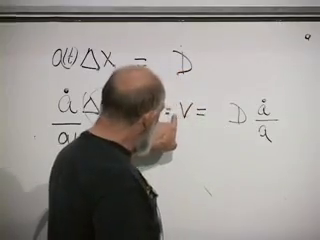
\includegraphics[width=0.73\textwidth]{lecture_08_figure_11.png}
\caption{物理的距離\(D=a\Delta x\)と、\(V=(\dot a/a)D\)に至るその時間微分。}
\lectureframe{01:16:45}
\end{figure}

\begin{classroomqa}
\audiencequestion{遠方の銀河に対して、ハッブルパラメータは現在の値で評価すべきか、それとも観測された光が放出された時点の値で評価すべきか。}
\lecturerresponse{記述されている時代の値で評価する。遠方の銀河からの光は、より早い時代の膨張の値を伝える。厳密な解析では\(H\)の時間依存性を考慮しなければならない。現在の値をどこにでも代入するのは局所近似にすぎない。}
\end{classroomqa}

\begin{classroomqa}
\audiencequestion{\(D=a\Delta x\)において単位はどこに存在するのか。}
\lecturerresponse{便利な選択は、共動ラベル\(\Delta x\)を無次元として扱い、\(a\)に長さを持たせることである。逆の記帳も可能である。いずれにせよ、\(H=\dot a/a\)は時間の逆数の次元を持つ。}
\end{classroomqa}

\section{膨張する座標における光}

光はヌル経路に従う。そのような経路に沿って固有時間間隔は消える：
\begin{equation}
  d\tau^2=0.
\end{equation}

\begin{classroomqa}
\audiencequestion{なぜ光に対して間隔はゼロなのか。}
\lecturerresponse{それが相対性理論における光線の定義的な幾何学である。すべての局所的自由落下観測者は光が\(c=1\)で進むと測定するので、局所的に\(dt^2=d\ell^2\)となり、時空間隔は消える。これは光を受け取る観測者に対して座標時間が経過しないという意味ではない。}
\end{classroomqa}

\(x\)方向のみに進む光線に対して、
\begin{equation}
  0=dt^2-a^2(t)\,dx^2.
\end{equation}
\(x\)が増加する向きに進む光線を選ぶと、
\begin{equation}
  dt=a(t)\,dx,
  \qquad
  dx=\frac{dt}{a(t)},
  \qquad
  \frac{dx}{dt}=\frac{1}{a(t)}.
  \label{eq:null-ray}
\end{equation}

\begin{figure}[H]
\centering
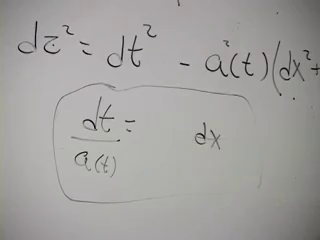
\includegraphics[width=0.64\textwidth]{lecture_08_figure_12.png}
\caption{膨張計量におけるヌル条件と、それから得られる共動光線方程式\(dx=dt/a(t)\)。}
\lectureframe{01:23:45}
\end{figure}

座標速度\(dx/dt\)はスケール因子が大きくなるにつれて減少する。これは光が局所的に遅くなるという意味ではない。1単位の共動座標距離はますます大きな物理的距離を表すので、座標速度の数値は変化するが、すべての局所測定は依然として\(c=1\)を与える。

\section{なぜ時間依存性が重要か}

中心的な幾何学の問いは今や避けられない：\(a(t)\)はどのように変化するのか。類推は、ある瞬間の位置がわかっている投射物である。その未来の軌道には運動方程式が必要である。宇宙論では、重力力学が\(a(t)\)の方程式を与えるであろう。

\begin{classroomqa}
\audiencequestion{なぜ\(a(t)\)が変化するかという問いを、たとえば電子電荷が時間とともに変化するかという同等に正当な問いよりも特権的に扱うのか。}
\lecturerresponse{論理的な階層は存在しない。電子電荷の測定された変化は極めて重要であろう。我々が\(a(t)\)に注目するのは、観測がすでに宇宙の間隔が変化することを教えているのに対し、電子電荷は一定に見えるからである。幾何学的には、一定の\(a\)は空間単位の変更によって除去でき、平坦な時空を残すであろう。時間依存の\(a\)はそのようには除去できない。}
\end{classroomqa}

遠方の後退を測定する前に、何が測定されているかを言うためにこの幾何学的枠組みが必要である。最も粗いレベルでは、既知の光度の光源は、その光がより大きな面積に広がるため距離とともに暗く見える。一方、既知の原子スペクトル線の変位は赤方偏移を与え、したがって後退の指標を与える。ハッブルは距離推定と赤方偏移を組み合わせて比例関係
\eqref{eq:hubble-law}
を明らかにしたが、係数の初期の数値はかなり誤っていた。現代の距離はしごと相対論的光伝播計算はずっと精巧であるが、概念的には距離と赤方偏移の対が依然として残る。

\section{ハッブル時間と年齢の推定}

ハッブルの法則には簡単な推定が隠れている。銀河の現在の後退速度を凍結し、運動を一様に逆向きに走らせる。現在の距離を閉じるのに必要な時間は
\begin{equation}
  t=\frac{D}{V}.
\end{equation}
となる。\(V=HD\)を用いると、
\begin{equation}
  t=\frac{D}{HD}=\frac{1}{H}.
  \label{eq:hubble-time}
\end{equation}
となる。距離が相殺されるので、共動銀河のどの対も同じ粗い時間を与える。ススキンドはここで容易な言葉の誤りを捉えて訂正する。仮定は\(H\)が一定に留まるということではない。特定の後退速度が、あたかも一定であるかのように逆向きに外挿されるということである。

\begin{figure}[H]
\centering
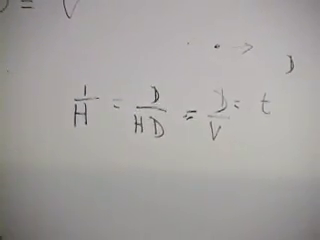
\includegraphics[width=0.66\textwidth]{lecture_08_figure_13.png}
\caption{ハッブル時間の推定値\(H^{-1}=D/(HD)=D/V\)では、後方外挿から距離が相殺される。}
\lectureframe{01:33:45}
\end{figure}

したがって、ハッブルパラメータの逆数は時間スケールであり、自動的に宇宙の正確な年齢になるわけではない。純粋に減速する物質優勢の描像では、現在の速度を逆転させ、重力が銀河を引き寄せるままにする。それらは等速の場合よりも早く出会うので、現在の\(H^{-1}\)は年齢を過大評価する。講義では約\(13.5\)億年という精密化された年齢が引用されており、ハッブル時間に近いが同一ではない。

\begin{classroomqa}
\audiencequestion{我々の銀河の内部にハッブル膨張がないなら、すべての銀河を崩壊するまで逆にたどるとはどういう意味か。}
\lecturerresponse{一様な記述は、最終的に束縛構造の実際の歴史を分解できなくなる。時間を前方に進めると、小さな揺らぎが重力的に成長して銀河や銀河団になる。文字通り逆再生した映画では、あらゆる微視的運動が逆転し、エントロピーが減少する必要がある。平均的なハッブル流れを単に逆転しても、構造形成が元に戻るわけではない。後方外挿は粗い宇宙論的推定であり、すべての恒星がその軌跡をたどる映画ではない。}
\end{classroomqa}

\begin{classroomqa}
\audiencequestion{実験は、膨張する銀河間距離と縮む物差しを区別できるか。}
\lecturerresponse{観測可能なのは無次元の比だけである。測定されるのは、銀河間の距離を原子または実験室の長さ標準で割った値が増加することである。我々は慣例的に原子・分子物理学のパラメータを固定して保持し、宇宙が膨張すると言う。銀河間の間隔を標準として選び、原子、陽子、メートル棒が縮んでいると記述することもできる。その比の物理学は変わらない。}
\end{classroomqa}

その慣例が自然なのは、棒が原子からできており、その大きさが一定に見えるパラメータによって制御されているからである。メートルは最終的に多数の微視的長さである。それらの微視的標準を固定して保持すると、\(a(t)\)が増大するというよく知られた言明が得られる。

\begin{classroomqa}
\audiencequestion{\eqref{eq:flrw-flat}は空間的一様性と平坦性に適合する唯一の計量か。}
\lecturerresponse{座標変換を除いてのみである。正確な主張は、それらの仮定と宇宙時間および共動空間座標の適切な選択の下で、計量をこの形に持ち込めるということである。別の座標系では、同じ時空がかなり異なって見えるかもしれない。}
\end{classroomqa}

\begin{classroomqa}
\audiencequestion{後方への分離がゼロに達すると、ハッブル則も速度ゼロを与える。それは銀河が出会うのを妨げるか。}
\lecturerresponse{いいえ。今日推測される\(H\)は、最後まで固定して保持されるわけではない。通常の膨張解では、\(H(t)\)はより初期の時刻にはるかに大きかった。推定値\(H_0^{-1}\)は、スケールを得るためだけに今日の速度を一様に延長して作られる。実際の\(a(t)\)、\(H(t)\)、速度は力学から求めなければならない。}
\end{classroomqa}

\section{ニュートンの球殻定理と宇宙論的力学}

力学を明らかにするには、銀河を一様な媒質に塗りつぶす。一つの銀河を原点として選び、別の銀河を共動ラベル\(x\)で指定する。この選択に物理的な特権はない。一様性は、最終的な方程式がすべての銀河の周りで同じであることを要求する。二番目の銀河の物理的半径は
\begin{equation}
  R(t)=a(t)x.
  \label{eq:radius-ax}
\end{equation}

最初は、その重力加速度を求めるには、巨大な宇宙にあるすべての銀河の引力を足し合わせる必要があるように思われる。ニュートンの球殻定理は問題を次のように崩壊させる。

\begin{proposition}[Newton's shell theorem]
逆二乗則の力と球対称な質量分布に対して、試験点を通る球の外側の物質は正味の力をゼロしか寄与しない。球の内側の物質は、囲まれた質量がすべて中心に集中しているかのように試験点に作用する。
\end{proposition}

\begin{figure}[H]
\centering
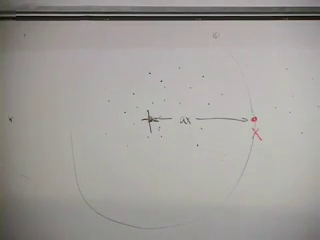
\includegraphics[width=0.70\textwidth]{lecture_08_figure_14.png}
\caption{一様な銀河分布、共動ラベル\(x\)にある試験銀河、およびその動径運動を囲まれた質量のみが制御する球。}
\lectureframe{01:50:05}
\end{figure}

\begin{figure}[H]
\centering
\begin{tikzpicture}[scale=0.94,>=Latex]
  \draw[gray!65] (0,0) circle (2.35);
  \foreach \p in {
    (-1.5,0.8),(-1.2,-0.8),(-0.8,1.5),(-0.6,0.35),(-0.3,-1.45),
    (0.15,1.05),(0.35,-0.55),(0.7,1.65),(0.9,0.45),(1.25,-0.9),
    (1.65,0.95),(-1.75,-0.2),(1.8,-0.15)} {
    \fill[black!55] \p circle (1.15pt);
  }
  \fill[blue!65!black] (0,0) circle (2pt)
    node[below left] {chosen origin};
  \fill[red!70!black] (2.35,0) circle (2.2pt)
    node[right] {test galaxy};
  \draw[->,thick] (0,0) -- (2.32,0)
    node[midway,above] {\(R=a(t)x\)};
  \draw[<->] (-2.35,-2.55) -- (2.35,-2.55)
    node[midway,below=4pt] {only the enclosed mass contributes};
\end{tikzpicture}
\caption{球殻定理の設定の明快な再構成。原点は便利な選択であり、宇宙の中心ではない。}
\end{figure}

したがって宇宙論的多体問題は、おなじみの一体問題となった。すなわち、現在の球の内部に閉じ込められた質量の引力の下で動径方向に運動する投射体である。ニュートンの方程式が、\(R=a x\) が、ひいては \(a(t)\) がどのように加速するかを決定する。講義はその計算を実行する前に意図的に止まっている。次回は、最も単純な物質優勢宇宙論を導出するのであって、その答えを幾何学的設定に密輸入するのではない。

\section{遅れて出た質問：光、ビッグバン、曲率}

正式な講義は終わったが、最後の質問はいくつかの誤解を招く描像を明らかにするものであり、付録ではなく物理学の一部である。

\begin{classroomqa}
\audiencequestion{非常に遠方の天体からの光が、宇宙がはるかに小さかったときに放出されたのなら、なぜそれは今、それほど遠くから来ているように見えるのか。また、初期宇宙がコンパクトだったのなら、なぜそのすべてが観測可能ではないのか。}
\lecturerresponse{膨張座標におけるヌル光線方程式を解かねばならない。\(a(t)\) が非常に小さいとき、\(dx/dt=1/a(t)\) は非常に大きい。光は、局所的には依然として \(c=1\) で進みながら、大きな共動区間を横切る。\(a(t)\) が大きくなるにつれて、その共動座標速度は減少する。正確な放出点と観測可能領域の大きさは、\(a(t)\) の全歴史に依存するので、数値的な答えは、特定の宇宙論が解かれるまで延期される。}
\end{classroomqa}

\begin{figure}[H]
\centering
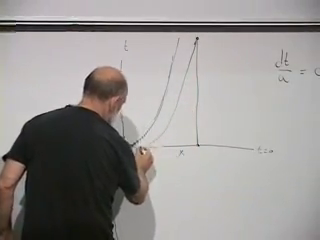
\includegraphics[width=0.72\textwidth]{lecture_08_figure_15.png}
\caption{\((x,t)\) 平面内の光線：\(a(t)\) が小さいとき共動座標ではほぼ水平であり、その後、スケール因子が大きくなるにつれて次第に急になる。}
\lectureframe{01:56:20}
\end{figure}

\eqref{eq:null-ray} を積分すると、延期された計算が明示的になる：
\begin{equation}
  \Delta x
  =\int_{t_{\mathrm e}}^{t_0}\frac{dt}{a(t)}.
  \label{eq:comoving-light-distance}
\end{equation}
\(t_{\mathrm e}\) が始まりに近づくにつれて積分が任意に大きな共動距離に達するかどうかは、\(a(t)\) の初期時間の形に依存する。\editorialnote{式 \eqref{eq:comoving-light-distance} は、黒板の式 \(dx=dt/a(t)\) の積分形である。それは、特定のスケール因子を選ぶことなく、講義が次回に割り当てる計算を明示的にする。}

\begin{figure}[H]
\centering
\begin{tikzpicture}[scale=0.92,>=Latex]
  \draw[->] (0,0) -- (6.4,0) node[right] {\(x\)};
  \draw[->] (0,0) -- (0,4.6) node[above] {\(t\)};
  \draw[thick,blue!65!black]
    plot[smooth] coordinates {(0,0.18) (1.65,0.42) (2.65,1.05)
      (3.35,2.05) (3.85,3.25) (4.05,4.25)};
  \fill[red!70!black] (4.05,4.25) circle (2pt)
    node[right] {reception today};
  \draw[dashed] (4.05,0) -- (4.05,4.25);
  \node[align=left] at (1.65,3.25)
    {\(\displaystyle \frac{dx}{dt}=\frac1{a(t)}\)\\
     large when \(a\) is small};
\end{tikzpicture}
\caption{共動座標における光線構成の整理された版。変化する傾きは座標効果であり、局所的な光速度の変化ではない。}
\end{figure}

\begin{classroomqa}
\audiencequestion{ビッグバンは物質を一点から放出したので、今では膨張する殻または環の上にあるべきなのか。}
\lecturerresponse{いいえ。このモデルは、一様で極めて高密度の空間から始まる。すべての大規模な間隔が成長する。物質は、優先的な中心から既存の空虚な空間を通って打ち出されるのではない。一様に点を付けた風船は有用な二次元の類推である。それが膨張するにつれて、すべての点の間隔が成長する一方、表面は一様に点で満たされたままである。空間はすべての正の時刻において無限でさえありうる。膨張は、それが何か他のものの内部の有限な球として始まったことを意味しない。}
\end{classroomqa}

\begin{classroomqa}
\audiencequestion{膨張の間、重力自体は弱かったのか、それとも強かったのか。}
\lecturerresponse{議論ではニュートンの定数 \(G\) を固定したままにする。それでも力は変化する。なぜなら間隔と閉じ込められた密度が変化するからである。以前は、同じ共動銀河は物理的により近く、一様な物質はより高密度だったので、重力による減速はより大きかった。これはまさに、球殻定理の計算が定量化しようとしているものである。}
\end{classroomqa}

最後に、空間曲率を膨張と混同してはならない。地球の小さな一片は、その大きさが地球の半径に比べて微小であるため平坦に見える。十分に大きな三角形を測定することにより、角度の超過を検出するか、曲率半径に下限を課すことができる。天文学は巨大な三角形を用いて同様の実験を行う。2006 年の講義で用いられた観測の言葉では、可視領域全体にわたって曲率は検出されなかったので、曲率半径はその領域より実質的に大きくなければならなかった。これは厳密に平坦な宇宙を証明するものではない。到達可能な部分がどれほど曲がりうるかに境界を与えるものである。

球について、内在的曲率は \(R^{-2}\) としてスケールする。したがって成長する球は局所的に平坦になる。同様に、一様な宇宙が非零の空間曲率をもつなら、膨張はその曲率半径を増大させ、任意の固定サイズの局所領域に見える曲率を減少させる。
\editorialnote{\(R^{-2}\) のスケーリングは、球が成長するにつれて数値的曲率が減少するという講義の記述の標準的な定量的形である。}

\begin{classroomqa}
\audiencequestion{もし空間が曲がっているなら、宇宙のある成分は収縮し、別の成分は膨張していなければならないのだろうか。}
\lecturerresponse{そうではない。正、ゼロ、負の空間曲率は、各宇宙時間スライスの幾何学を記述する。膨張または収縮は\(a(t)\)の時間発展によって支配される。曲がった宇宙は膨張しうるし、平坦な宇宙は収縮しうる。膨張は後に反転するかもしれない。ちょうど上向きに運動する投射物が落下して戻りうるように。しかし同時収縮が曲率の中に隠れているわけではない。力学上の問題は、外向きの運動が内部に含まれる質量の引力を振り切るか、落下して戻るか、それとも臨界境界上にあるかである。}
\end{classroomqa}

その脱出速度の比較が、この講義の最後の板書レベルの考えである。幾何学は計量、ハッブル則、光線方程式を与えた。ニュートンの定理は力学を一つの球の内部の質量に帰着させた。次の講義は、まさにこの講義が終わるべきところから始まる。すなわち、\(a(t)\)を決定する方程式から、そして膨張が振り切るのか、再収縮するのか、それとも刃の上に留まるのかという問いからである。
